\chapter{Graph Neural Networks}

\section{Little back to Convolutional Neural Networks}
\begin{wrapfigure}{r}{0.4\textwidth}
    \centering
    \vspace{-10pt}
    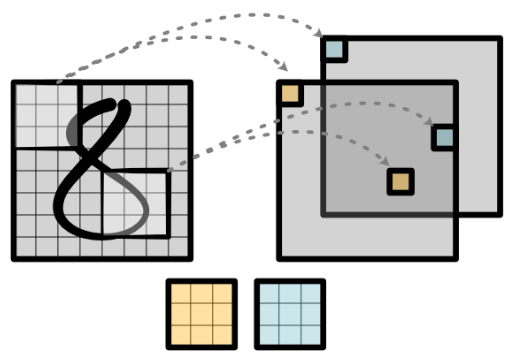
\includegraphics[width=\linewidth]{images/ex_conv.png}
    \label{fig:conv}
    \vspace{-10pt}
\end{wrapfigure}
The \textbf{2D spatial cross-correlation} between an input image $I$ and a square kernel $K \in R^{d \times d}$ is defined as:
\[
S(i, j) = \sum_{m=-k}^{k} \sum_{n=-k}^{k} I(i + m, j + n) \cdot K(m, n)
\]
where:
\begin{compactitemize}
    \item $d = 2k + 1$: kernel size (square)
    \item $I(i+m, j+n)$: pixel value at position $(i+m, j+n)$ in the input image
    \item $K(m, n)$: kernel weight
\end{compactitemize}

\subsection{1D Cross-Correlation on a 1D Euclidean Lattice} 
\begin{wrapfigure}{r}{0.5\textwidth}
    \centering
    \vspace{-10pt}
    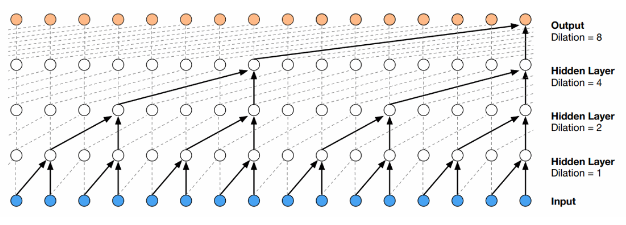
\includegraphics[width=\linewidth]{images/1D.png}
    \label{fig:conv1D}
    \vspace{-10pt}
\end{wrapfigure}
Just like in 2D, the 1D grid can be seen as a discretization of a continuous Euclidean line $\mathbb{R}$, sampled at regular intervals.  
In this case both input and kernel are defined on a 1D Euclidean space, and the kernel slides along this lattice, computing local interactions at each position.  
This setup is widely used in domains such as audio processing, NLP, and time series analysis.

\subsection{2D Cross-Correlation on a 2D Euclidean Lattice} 
The image can also be represented as a 2D grid graph, where each pixel is a node connected to its neighboring pixels. In particular:
\begin{compactitemize}
    \item Each pixel lies on a \textbf{discrete 2D lattice} $\mathbb{Z}^2$ embedded in Euclidean plane.
    \item Cross-correlation slides a small kernel across this grid, visiting each location systematically.
    \item At each location, the kernel interacts with a local patch, treating it as a \textbf{neighborhood in 2D space}.
\end{compactitemize}

\begin{figure}[H]
    \centering
    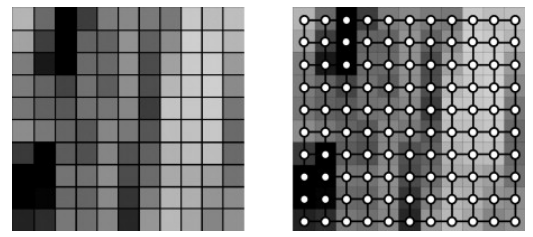
\includegraphics[width=0.5\textwidth]{images/image_graph.png}
    \caption{Image represented as a graph.}
    \label{fig:image_graph}
\end{figure}

\begin{infobox}[Note]
    Although the operation is discrete, the grid itself can be viewed as a sampling of a continuous 2D Euclidean space.
\end{infobox}

\subsection{A Graph Viewpoint}
Under this new viewpoint, the input image can be interpreted as a \textbf{signal lying on a (Euclidean) graph}.  
A graph $G = (V, E)$ consists of a set of nodes (vertices) $V$ and a set of edges $E \subseteq V \times V$.  
Graphs can be:
\begin{compactitemize}
    \item \textbf{Directed or undirected}
    \item \textbf{Weighted or unweighted}
\end{compactitemize}

A \textbf{lattice graph} is a particular case where nodes are arranged on a regular grid (e.g., 1D, 2D, or 3D).  
In the case of a 2D Euclidean lattice:
\begin{compactitemize}
    \item Each pixel corresponds to a node in the graph.
    \item Each node is associated with a feature vector (e.g., a triplet of raw RGB values).
    \item The edge set $E$ connects each node to its spatial neighbors using a fixed connectivity rule (e.g., 4-connected: top, bottom, left, right).
\end{compactitemize}

\subsection{Problem of Standard N-D Convolution}
A limitation of traditional convolutional architectures is that they assume data is defined over \textbf{regular Euclidean grids} (e.g., 1D signals, 2D images).  
These models rely on:
\begin{compactitemize}
    \item \textbf{Fixed neighborhood structures}, determined by the lattice topology.
    \item \textbf{Shift-invariance} properties, which hold only in regular domains.
\end{compactitemize}

However, many real-world data domains — such as social networks, molecular structures, and transportation systems — are inherently \textbf{non-Euclidean}.  
This motivates the need for generalizing convolutional operations to arbitrary graph structures, leading to the development of \textbf{Graph Neural Networks (GNNs)}.

\begin{figure}[H]
    \centering
    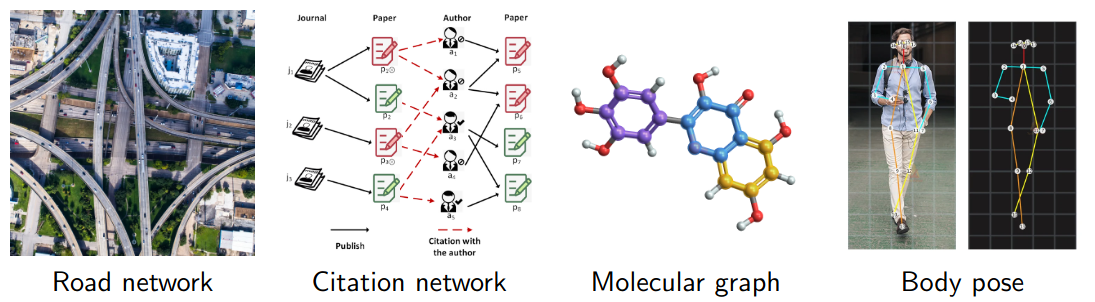
\includegraphics[width=0.9\textwidth]{images/non_euclidian_domains.png}
    \caption{Example of no Euclidian Domains.}
    \label{fig:image_graph}
\end{figure}

\section{Graph Neural Networks}
The objective of Graph Neural Networks (GNNs) is to define a NN that can handle \textbf{graph-structured data}. In particular a NN that can handle:
\begin{compactitemize}
    \item \textbf{Irregular structures}: node may have different number of neighbors (no fixed-size receptive field).
    \item \textbf{No spatial locality}: unlike images, there is no inherent notion of distance or order between nodes.
    \item \textbf{Permutation invariance}: the model's output should not depend on the order in which nodes are processed.  So if we have two identical graphs, but with different node ordering, the output should be the same.
    \WFclear
    \item \textbf{No global coordinate system}: we cannot rely on a fixed layout or orientation.
    \item \textbf{Dynamic topology}: edge connectivity may evolve or depend on node features.
\end{compactitemize}
\begin{figure}[H]
    \centering
    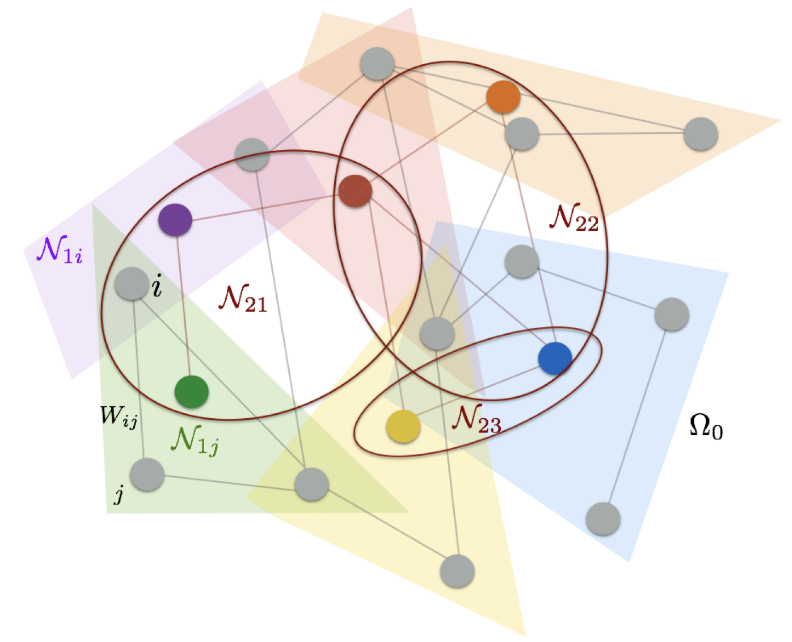
\includegraphics[width=0.3\textwidth]{images/graph_data.png}
    \caption{Graph data structured.}
    \label{fig:image_graph}
\end{figure}

\textbf{Graph Convolutional Networks} introduced by Kipf and Welling generalize convolution to graph-structured data convolution to graph-structured data. As with standard neural network like MLPs and CNNs:
\begin{compactitemize}
    \item A GNNs is structured in multiple succesive layers.
    \item We have input features, hidden activations (often call \textbf{node embeddings}), activation functins and output responses.
    \item Gradient descent and backpropagation are used to train the model.
\end{compactitemize}


A key idea of GCNs is to define a \textbf{message-passing}, where each node updates its feature representation by aggregating information from its neighbors. The processes follow these steps:
\begin{wrapfigure}{r}{0.5\textwidth}
    \centering
    \vspace{-10pt}
    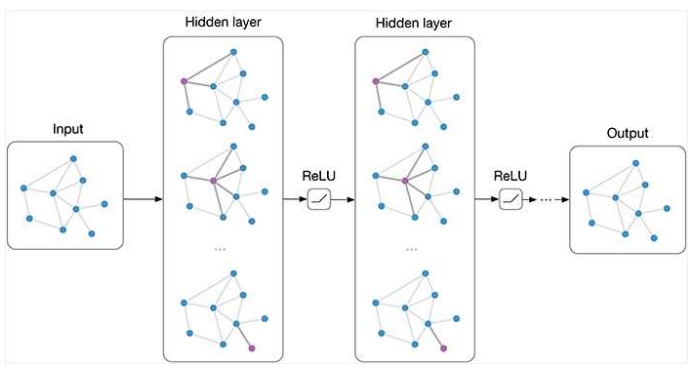
\includegraphics[width=\linewidth]{images/GNN.png}
    \label{fig:conv1D}
    \vspace{-10pt}
\end{wrapfigure}
\begin{compactitemize}
    \item \textbf{Step 1}: Leveraging the graph structure, each node collects information from its neighbors by combining their embeddings. The embeddings are combined through an aggregation (poolin) function (e.g., sum, mean, max).
    \item \textbf{Step 2}: The aggregated information is then passed through a neural network layer (e.g, a simple MLP) to generate a new representation (embedding) for the node. This results in an  \textbf{updated node representation} that captures both its own features and those of its local neighborhood.
\end{compactitemize}

\begin{infobox}[How Graph Convolutional Layer Works]
    \textbf{Input for each node $v$:}
\begin{compactitemize}
    \item Node's own feature vector: $\mathbf{h}_v^{(l)}$ (embedding at layer $l$)
    \item Neighbor feature vectors: $\{\mathbf{h}_u^{(l)} : u \in \mathcal{N}(v)\}$ where $\mathcal{N}(v)$ is the set of neighbors
\end{compactitemize}

\textbf{Computation steps:}
\begin{enumerate}
    \item \textbf{Aggregation}: Combine neighbor features
    $$\mathbf{m}_v^{(l)} = \text{AGGREGATE}\left(\{\mathbf{h}_u^{(l)} : u \in \mathcal{N}(v)\}\right)$$
    Common aggregation functions:
    \begin{compactitemize}
        \item Sum: $\mathbf{m}_v = \sum_{u \in \mathcal{N}(v)} \mathbf{h}_u^{(l)}$
        \item Mean: $\mathbf{m}_v = \frac{1}{|\mathcal{N}(v)|} \sum_{u \in \mathcal{N}(v)} \mathbf{h}_u^{(l)}$
        \item Max: $\mathbf{m}_v = \max_{u \in \mathcal{N}(v)} \mathbf{h}_u^{(l)}$
    \end{compactitemize}
    
    \item \textbf{Update}: Combine aggregated message with node's own features
    $$\mathbf{h}_v^{(l+1)} = \sigma\left(\mathbf{W}^{(l)} \cdot \text{CONCAT}(\mathbf{h}_v^{(l)}, \mathbf{m}_v^{(l)}) + \mathbf{b}^{(l)}\right)$$
    where $\mathbf{W}^{(l)}$ is a learnable weight matrix, $\mathbf{b}^{(l)}$ is a bias, and $\sigma$ is an activation function (e.g., ReLU).
\end{enumerate}

\textbf{Output}: Updated node embedding $\mathbf{h}_v^{(l+1)}$ that incorporates information from the local neighborhood.
\end{infobox}

\subsection{An example of Graph Convolutional Layer}
\begin{wrapfigure}{r}{0.3\textwidth}
    \centering
    \vspace{-10pt}
    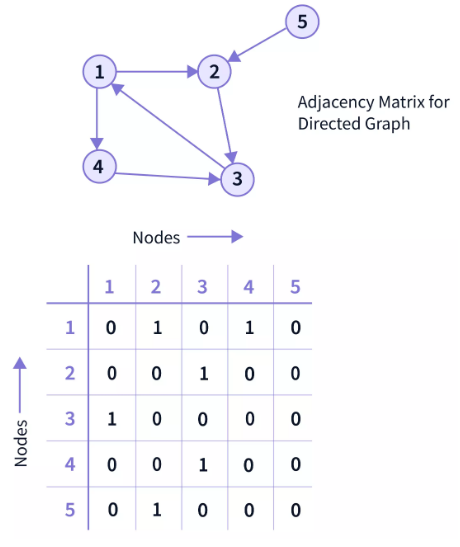
\includegraphics[width=\linewidth]{images/GCN_example.png}
    \label{fig:conv1D}
    \vspace{-10pt}
\end{wrapfigure}
GCN Layer (Kipf and Welling, 2017) represents one of the most prominent examples of graph-based neural netowrks. The net has two input:
\begin{compactitemize}
    \item \textbf{Node features matrix} $X \in R^{nxd}$: each row corresponds to the feature vector of a node.
    \item \textbf{Adjacency matrix} $A \in R^{nxn}$: encodes the graph structure, where $A_{ij} = 1$ if there is an edge from node $i$ to node $j$, and $0$ otherwise. This if the matrix is binary, but it can also be weighted.
\end{compactitemize}

\subsection{The Role of the Adjacency Matrix}
The \textbf{adjacency matrix} $\mathbf{A}$ is a fundamental component of Graph Neural Networks, serving multiple critical roles in the learning process. First, it acts as a \textbf{structural prior} that encodes the geometry and topology of the underlying domain. By explicitly representing which nodes are connected, the adjacency matrix provides the model with essential information about the spatial or relational structure of the data, allowing the GNN to respect and leverage these constraints during feature propagation. This is particularly important because, unlike grid-structured data (e.g., images), graphs lack inherent spatial regularity, and the adjacency matrix compensates for this by defining the neighborhood structure explicitly.

Beyond encoding structure, the adjacency matrix plays a crucial role in \textbf{regularization and generalization}. By limiting message passing to only those connections defined in $\mathbf{A}$, the model enforces locality, meaning that information flow is restricted to meaningful, structurally-relevant paths rather than allowing unconstrained communication between all nodes. This locality constraint acts as a powerful form of inductive bias that helps prevent overfitting: the model cannot learn arbitrary dependencies between distant or unrelated nodes, but must instead focus on learning patterns that respect the graph's topology. This injection of domain-specific structure into the model architecture enables better generalization to unseen graphs with similar structural properties, as the learned features are inherently tied to the relational structure rather than being purely data-driven.

The adjacency matrix can be obtained or constructed through various approaches, depending on the application:

\begin{compactitemize}
\item \textbf{Domain knowledge}: The graph structure is defined manually based on expert knowledge of the problem domain. Examples include human skeleton graphs where edges connect anatomically-linked joints, molecular graphs where edges represent chemical bonds between atoms, or citation networks where edges indicate references between papers.

\item \textbf{Heuristic construction}: When the graph structure is not explicitly given, it can be constructed using data-driven heuristics. Common approaches include:
\begin{compactitemize}
\item \textit{k-nearest neighbors (k-NN)}: Connect each node to its $k$ closest neighbors in feature space, typically using Euclidean distance or cosine similarity.
\item \textit{Distance thresholds}: Create edges between nodes whose feature vectors are within a specified distance threshold $\epsilon$.
\item \textit{Similarity-based}: Define edge weights based on feature similarity, creating a weighted adjacency matrix where $A_{ij} = \text{sim}(\mathbf{x}_i, \mathbf{x}_j)$.
\end{compactitemize}
\end{compactitemize}

\subsection{Message Passing}
The core operation of Graph Convolutional Networks (GCNs) is defined by a \textbf{layer-wise propagation rule} that updates node embeddings by aggregating information from their neighborhoods. The mathematical formulation of this process is given by:

$$\mathbf{H}^{(l)} = \sigma\left(\hat{\mathbf{D}}^{-\frac{1}{2}} \hat{\mathbf{A}} \hat{\mathbf{D}}^{-\frac{1}{2}} \mathbf{H}^{(l-1)} \mathbf{W}^{(l)}\right)$$

where the key components are:

\begin{compactitemize}
\item $\hat{\mathbf{A}} = \mathbf{A} + \mathbf{I}$: the adjacency matrix with added self-loops. The addition of the identity matrix $\mathbf{I}$ ensures that each node also considers its own features during aggregation, not just those of its neighbors.

\item $\hat{\mathbf{D}}$: the degree matrix of $\hat{\mathbf{A}}$, defined as a diagonal matrix where $\hat{D}_{i,i} = \sum_j \hat{A}_{i,j}$. This matrix captures how many connections (including the self-loop) each node has.

\item $\hat{\mathbf{D}}^{-\frac{1}{2}} \hat{\mathbf{A}} \hat{\mathbf{D}}^{-\frac{1}{2}}$: the symmetric normalization of the adjacency matrix. This normalization is crucial because it prevents nodes with many neighbors from having disproportionately large feature values, ensuring numerical stability and balanced information flow.

\item $\mathbf{H}^{(l-1)} \in \mathbb{R}^{|V| \times F_{l-1}}$: the matrix of node embeddings from the previous layer, where $|V|$ is the number of nodes and $F_{l-1}$ is the feature dimension at layer $l-1$.

\item $\mathbf{W}^{(l)} \in \mathbb{R}^{F_{l-1} \times F_l}$: a learnable projection matrix that transforms features from dimension $F_{l-1}$ to $F_l$. This is the trainable component of the layer.

\item $\sigma(\cdot)$: a non-linear activation function (e.g., ReLU) that introduces non-linearity into the model.
\end{compactitemize}

\textbf{Alternative per-node formulation:} For binary adjacency matrices, the GCN operation can be expressed at the individual node level, which provides clearer intuition about the message-passing mechanism:

\begin{enumerate}
\item \textbf{Aggregation}: Each node $v$ collects and normalizes features from its neighbors (including itself):
$$\mathbf{a}_v^{(l)} = \sum_{u \in \mathcal{N}(v) \cup \{v\}} \frac{1}{\sqrt{\hat{d}_v \hat{d}_u}} \mathbf{h}_u^{(l-1)}$$
where $\hat{d}_v$ and $\hat{d}_u$ are the degrees of nodes $v$ and $u$ in $\hat{\mathbf{A}}$. The normalization factor $\frac{1}{\sqrt{\hat{d}_v \hat{d}_u}}$ ensures that nodes with many neighbors don't dominate the aggregation.

\item \textbf{Projection}: The aggregated features are linearly transformed:
$$\mathbf{z}_v^{(l)} = \mathbf{a}_v^{(l)} \cdot \mathbf{W}^{(l)}$$

\item \textbf{Non-linearity}: An activation function is applied to produce the final updated embedding:
$$\mathbf{h}_v^{(l)} = \sigma(\mathbf{z}_v^{(l)})$$
\end{enumerate}

This formulation makes explicit that each node's embedding is updated using features from $\mathcal{N}(v)$ (the set of its immediate neighbors $u$, each with its degree $\hat{d}_u$) and from itself, with appropriate normalization based on the connectivity structure.

\subsubsection{Receptive Field and Theoretical Motivations}
A single GCN layer performs aggregation over the \textbf{first-order neighborhood}, meaning it only considers nodes that are directly connected (1-hop neighbors). However, by stacking multiple GCN layers, the model can capture information from increasingly distant parts of the graph. Specifically, an $L$-layer GCN has a receptive field of $L$ hops: after $L$ layers, each node's representation incorporates information from all nodes within $L$ steps in the graph. For example, a 2-layer GCN for node classification can be written as:

$$\mathbf{Z} = \text{softmax}\left(\hat{\mathbf{D}}^{-\frac{1}{2}} \hat{\mathbf{A}} \hat{\mathbf{D}}^{-\frac{1}{2}} \sigma\left(\hat{\mathbf{D}}^{-\frac{1}{2}} \hat{\mathbf{A}} \hat{\mathbf{D}}^{-\frac{1}{2}} \mathbf{X} \mathbf{W}^{(0)}\right) \mathbf{W}^{(1)}\right)$$

where $\mathbf{X}$ is the input feature matrix, and the final softmax produces class probabilities for node classification tasks.

The GCN architecture is not just an empirical design but has solid theoretical foundations rooted in spectral graph theory. Specifically, the GCN can be understood as a first-order approximation of spectral graph convolutions, which are based on the spectral formulation of convolution operations on graphs. This connection to spectral theory provides mathematical justification for why the normalized adjacency matrix and the specific aggregation scheme lead to effective learning on graph-structured data.

\section{Applications of Graph Neural Networks}

\subsection{Node Classification}
The task is predict a label for each node in the graph, in details:
\begin{compactitemize}
    \item Each node $v \in V$ has an input feature vector $\mathbf{x}_v$.
    \item Through multiple layers, the GNN encodes it into a node embedding $h_v \in R^d$.
    \item A classification layer maps the embedding to class scores:
    \[
        z_v = W h_v + b \in R^C
    \]
    \item The predicted label is then:
    \[
        \hat{y}_v = \text{argmax}_c z_{v}[c]
    \]
\end{compactitemize}
The output is $Z \in R^{NxC}$

The are two main settings:
\begin{compactitemize}
    \item \textbf{Transductive Setting}: The entire graph is available during training, but labels are known only for a subset of nodes. The goal is to predict label for the remaining nodes in the same graph. The model can be leverage connections to all nodes (labeled and enlabeled). Unlabeled nodes influence learning through shared structure, even if not supervised directly.
    \item \textbf{Inductive Setting}: The model must generalize to \textbf{unseen nodes or graphs.} These nodes are not part of the training graph. Predictions rely only on node features and local structure. The model learns representations that transfer across graphs.
\end{compactitemize}

\begin{figure}[H]
    \centering
    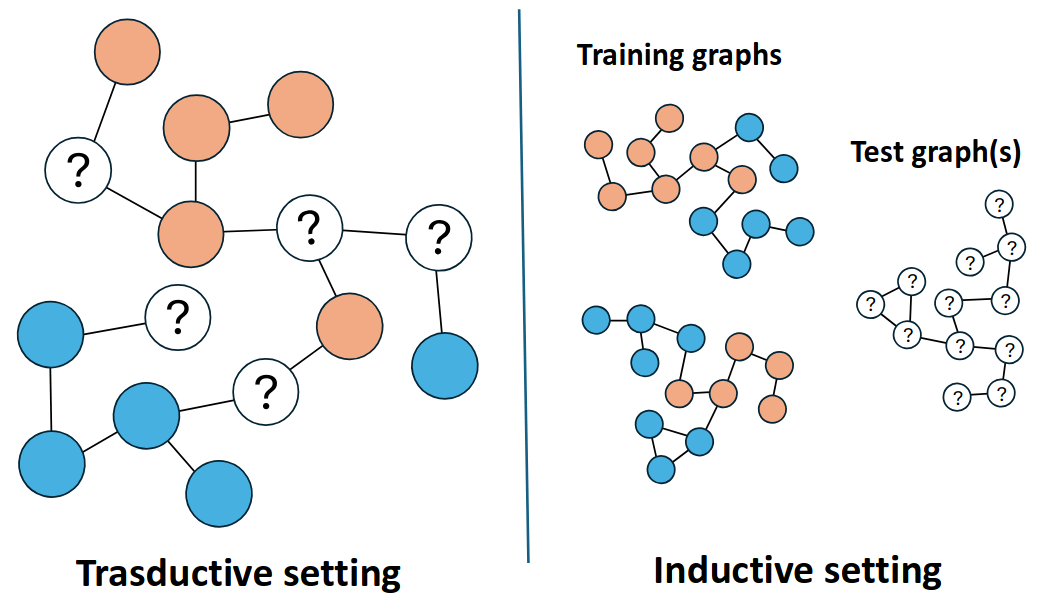
\includegraphics[width=0.6\textwidth]{images/node_classification.png}
    \caption{Node classification settings.}
    \label{fig:image_graph}
\end{figure}

\subsection{Link Prediction}
The task is to predict the existence of edges between pairs of nodes. In details:
\begin{compactitemize}
    \item Given two nodes $u$ and $v$, the goal is to predict if $(u, v) \in E$
    \item This is a binary classification task on node pairs (or multi-class for edge types).
    \item Common pipeline:
    \begin{compactitemize}
        \item Learn node embeddings $h_u$ and $h_v$ via GNN.
        \item Compute edge representation:
        \[
            s_{uv}=Decoder(h_u, h_v)
        \]
        \item Map to class scores:
        \[
            z_{uv} = W s_{uv} + b \in R^C
        \]
        \item Predict edge existence:
        \[
            \hat{y}_{uv} = \text{argmax}_c z_{uv}[c]
        \]
    \end{compactitemize}
\end{compactitemize}

Applications include:
\begin{compactitemize}
    \item Social network link prediction (friend recommendations)
    \item Biological networks: Predict protein-protein or drug-target interactions.
    \item Recommender systems (user-item interactions)
\end{compactitemize}

\subsection{Graph Classification}
The task is to predict a label for an entire graph. In details:
\begin{compactitemize}
    \item Each graph $G_i = (V,E)$ is treated as a single data point.
    \item Node features are processed by GNN layers to obtain node embeddings $h_v$.
    \item A textbf{global pooling} functions aggregates them into a single graph-level vector:
    \[
        h_{graph} = \text{POOLING}(\{h_v | v \in V\})
    \]
\end{compactitemize}
A finale MLP predicts the graph label:
\[
    \hat{y}_{G}=MLP(h_{graph})
\]
The pooling function can be:
\begin{compactitemize}
    \item \textbf{Global Average Pooling}: $h_{graph} = \frac{1}{|V|} \sum_{v \in V} h_v$
    \item \textbf{Attention-based Pooling}: $h_{graph} = \sum_{v \in V} \alpha_v h_v$  with $\alpha_v = softmax(a^T h_v)$
\end{compactitemize}
While these two approaches summurize the entire set of vertices in a single step, other methods allow for hierarchical pooling, similar to what is done in standard CNNS.

\begin{figure}[H]
    \centering
    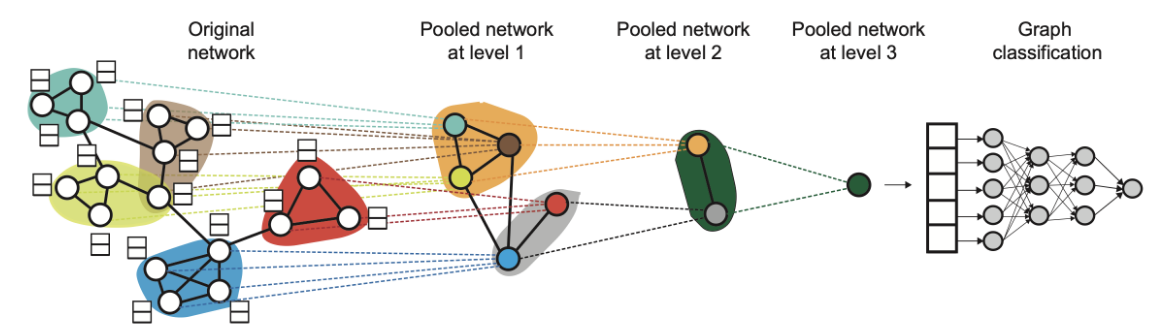
\includegraphics[width=0.9\textwidth]{images/hierarchical_pooling.png}
    \caption{Example of hierarchical pooling.}
    \label{fig:image_graph}
\end{figure}

\begin{wrapfigure}{r}{0.3\textwidth}
    \centering
    \vspace{-10pt}
    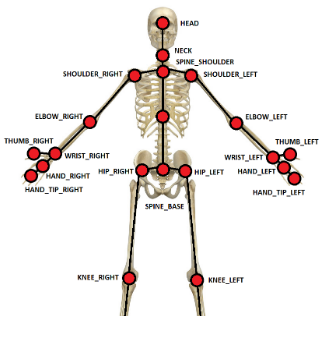
\includegraphics[width=\linewidth]{images/scheletro.png}
    \label{fig:conv1D}
    \vspace{-10pt}
\end{wrapfigure}
A classic application of graph classification is \textbf{Action Recognition}. Given a sequence of human poses represented as skeleton graphs, the goal is to classify the action being performed (e.g., walking, running, jumping). 
Graphs are constructed with:
\begin{compactitemize}
    \item \textbf{Spatial edges}: connections between joints.
    \item \textbf{Temporal edges}: same joint across frames.
\end{compactitemize}
The GNNs or Spatio-Temporal GCNs (ST-GCNs) are used to.


\begin{figure}[H]
    \centering
    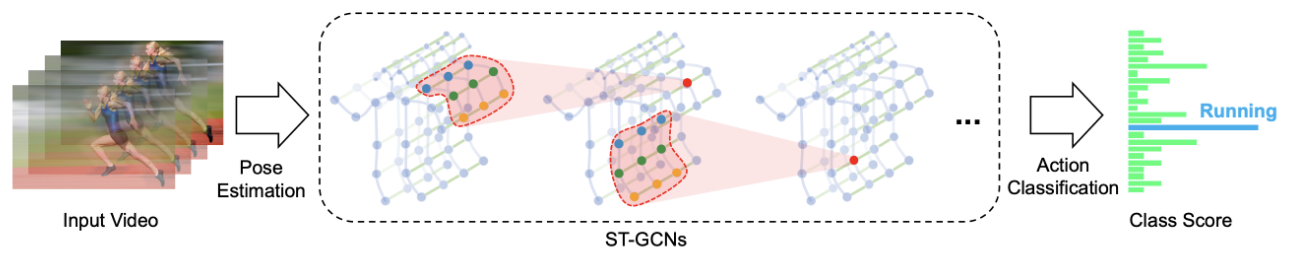
\includegraphics[width=0.9\textwidth]{images/Action.png}
    \caption{Example of action recognition.}
    \label{fig:image_graph}
\end{figure}


\section{Graph Attention Networks (GATs)}

\subsection{Limitations of GCNs}

While Graph Convolutional Networks provide a powerful framework for learning on graph-structured data, they suffer from several fundamental limitations that restrict their expressiveness and practical applicability. Recall the layer-wise propagation rule of GCN:

$$\mathbf{H}^{(l)} = \sigma\left(\hat{\mathbf{D}}^{-\frac{1}{2}} \hat{\mathbf{A}} \hat{\mathbf{D}}^{-\frac{1}{2}} \mathbf{H}^{(l-1)} \mathbf{W}^{(l)}\right)$$

The main problems with this formulation are:

\begin{compactitemize}
\item \textbf{Over-smoothing}: As the number of layers increases, node representations tend to become increasingly similar and eventually indistinguishable. This happens because repeated neighborhood averaging causes all nodes to converge toward similar feature distributions, losing the discriminative power needed for downstream tasks. This severely limits the depth of GCN architectures.

\item \textbf{Uniform aggregation}: All neighbors contribute equally (or only degree-normalized) to a node's representation, without any adaptive weighting or attention mechanism. The model cannot distinguish between important and less important neighbors—every connection in the graph is treated with the same significance, regardless of the actual relevance of the information being passed.

\item \textbf{Limited expressivity}: GCNs are heavily dependent on the structure encoded in the input adjacency matrix $\mathbf{A}$. The model cannot adapt or learn which connections are truly important for the task at hand; it is constrained by the pre-defined graph topology. If the adjacency matrix does not accurately reflect the relationships relevant to the learning task, the GCN's performance will be fundamentally limited.
\end{compactitemize}

These limitations motivate the development of more flexible architectures that can learn adaptive, task-specific edge weights rather than relying solely on the fixed graph structure.

\subsection{Graph Attention Networks: Core Idea}
Graph Attention Networks (GATs), introduced by Veličković et al., address the limitations of GCNs by incorporating an \textbf{attention mechanism} that allows the model to learn which neighbors are most relevant for each node. The key innovations of GATs are:
\begin{compactitemize}
\item \textbf{Learned edge weights}: The model learns adaptive attention coefficients that determine how much each neighbor contributes to a node's updated representation. This eliminates the need for pre-defined weighted adjacency matrices, as the importance of each connection is learned from data.
\item \textbf{Local adaptivity}: Different neighbors of the same node can receive different attention weights, allowing the model to focus on the most informative connections. This enables more flexible and expressive aggregation compared to the uniform (or degree-normalized) weighting in GCNs.
\item \textbf{Structural awareness}: Through the attention mechanism, each node selectively attends to its neighboring nodes as defined by the input adjacency matrix. However, unlike GCNs, the strength of these connections is not fixed but rather learned during training, making the model more robust to noise or irrelevant edges in the graph structure.
\end{compactitemize}
The attention mechanism allows GATs to automatically identify which neighbors carry the most relevant information for updating each node's features, leading to more discriminative representations and better performance on graph learning tasks.

\subsection{GAT Architecture: Detailed Mechanism}

The GAT layer computes updated node representations through a sequence of operations that combine linear transformations with learned attention weights. The process can be broken down into the following steps:

\begin{compactitemize}
\item \textbf{Step 1: Linear Projection.} First, a shared linear transformation is applied to all node features to project them into a new feature space:
$$\mathbf{h}_i^W = \mathbf{W}\mathbf{h}_i \quad \text{for each node } i$$
where $\mathbf{W} \in \mathbb{R}^{F' \times F}$ is a learnable weight matrix that projects features from dimension $F$ to dimension $F'$. This transformation is shared across all nodes, similar to the projection in GCNs, and allows the model to learn task-relevant feature representations.

\item \textbf{Step 2: Attention Score Computation.} Next, the model computes an unnormalized attention score (or affinity score) between node $i$ and each of its neighbors $j$:
$$e_{ij} = \text{LeakyReLU}\left(\mathbf{a}^\top [\mathbf{h}_i^W \| \mathbf{h}_j^W]\right)$$
where $[\cdot \| \cdot]$ denotes vector concatenation, $\mathbf{a} \in \mathbb{R}^{2F'}$ is a learnable weight vector that parameterizes the attention mechanism, and LeakyReLU is the activation function applied to introduce non-linearity. The concatenation $[\mathbf{h}_i^W \| \mathbf{h}_j^W]$ creates a $2F'$-dimensional vector that captures both the features of the central node $i$ and its neighbor $j$. The learned vector $\mathbf{a}$ then computes a scalar attention score that indicates how important neighbor $j$'s features are to node $i$. Importantly, this attention score is \textbf{asymmetric}: the importance of $j$ to $i$ (captured by $e_{ij}$) may differ from the importance of $i$ to $j$ (captured by $e_{ji}$), allowing the model to capture directed relationships even in undirected graphs.

\item \textbf{Masked Attention.} In its most general formulation, the attention mechanism could allow every node to attend to every other node in the graph, which would discard all structural information encoded in the adjacency matrix. To preserve the graph structure, GATs employ \textbf{masked attention}: the attention score $e_{ij}$ is computed only for nodes $j \in \mathcal{N}(i)$, where $\mathcal{N}(i)$ denotes the first-order neighbors of node $i$ (including $i$ itself, if self-loops are used). This way, the graph topology acts as a mask that restricts attention to structurally connected nodes, while still allowing the model to learn the relative importance of these connections. An important advantage of masked attention is that \textbf{the graph need not be undirected}: if an edge $j \to i$ is not present in the adjacency matrix, the computation of $\alpha_{ij}$ is simply omitted. This makes GATs naturally applicable to directed graphs without requiring symmetrization.

\item \textbf{Step 3: Attention Normalization.} The unnormalized attention scores are then normalized across all neighbors of node $i$ using a softmax function:
$$\alpha_{ij} = \frac{\exp(e_{ij})}{\sum_{k \in \mathcal{N}(i)} \exp(e_{ik})}$$
This normalization ensures that the attention coefficients $\alpha_{ij}$ sum to 1 across all neighbors, making them interpretable as the relative importance of each neighbor. The softmax operation also ensures numerical stability and makes the attention coefficients differentiable, allowing end-to-end training via backpropagation.

\item \textbf{Step 4: Weighted Aggregation.} Finally, the updated node representation is computed as a weighted sum of the transformed neighbor features, where the weights are the learned attention coefficients:
$$\mathbf{h}_i' = \sigma\left(\sum_{j \in \mathcal{N}(i)} \alpha_{ij} \mathbf{h}_j^W\right)$$
where $\sigma$ is a non-linear activation function (e.g., ReLU or ELU). This aggregation is fundamentally different from GCNs: instead of using fixed (or degree-normalized) weights, each neighbor's contribution is modulated by the learned attention coefficient $\alpha_{ij}$, allowing the model to emphasize important neighbors and downweight less relevant ones.

\item \textbf{Step 5: Multi-Head Attention (optional).} To stabilize the learning process and increase the model's expressive power, GATs employ \textbf{multi-head attention}, similar to the mechanism used in Transformers. The idea is to execute $K$ independent attention mechanisms in parallel, each with its own learnable parameters $\mathbf{W}^{(k)}$ and $\mathbf{a}^{(k)}$. The outputs from all $K$ attention heads are then combined. For intermediate layers, the outputs are typically concatenated:
$$\mathbf{h}_i' = \|_{k=1}^K \sigma\left(\sum_{j \in \mathcal{N}(i)} \alpha_{ij}^{(k)} \mathbf{W}^{(k)} \mathbf{h}_j\right)$$
where $\|$ denotes concatenation and $\alpha_{ij}^{(k)}$ are the attention coefficients computed by the $k$-th attention head. Note that with $K$ heads, each producing $F'$-dimensional features, the final output $\mathbf{h}_i'$ will have dimension $KF'$ rather than $F'$. For the final layer (e.g., in classification tasks), averaging is typically used instead of concatenation:
$$\mathbf{h}_i' = \sigma\left(\frac{1}{K} \sum_{k=1}^K \sum_{j \in \mathcal{N}(i)} \alpha_{ij}^{(k)} \mathbf{W}^{(k)} \mathbf{h}_j\right)$$
Multi-head attention provides several benefits: it allows the model to attend to different aspects of the neighborhood simultaneously, reduces the risk of overfitting to specific attention patterns, and empirically leads to more stable training and better generalization.
\end{compactitemize}

\textbf{Additional enhancements:} Like many modern deep learning architectures, GATs can be combined with \textbf{residual connections} to facilitate gradient flow and enable training of deeper networks, further improving their expressiveness and mitigating over-smoothing issues.

\begin{table}[h]
    \centering
    \caption{Comparison between GAT and Self-Attention (Transformers)}
    \begin{tabular}{|p{3.5cm}|p{5.5cm}|p{5.5cm}|}
    \hline
    \textbf{Aspect} & \textbf{GAT} & \textbf{Self-Attention (Transformers)} \\
    \hline
    Input structure & Graph (nodes + edges) & Sequence (e.g., tokens) \\
    \hline
    Neighborhood & Defined by adjacency matrix & Full attention (every token attends to all others) \\
    \hline
    Sparsity & Sparse: only local neighbors & Dense: full pairwise interactions \\
    \hline
    Attention mechanism & Single-layer MLP over concatenated node pairs & Dot-product between learned query and key vectors \\
    \hline
    Position encoding & Implicit via graph topology & Explicit (e.g., sinusoidal or learned) \\
    \hline
    Inductive bias & Local, relational inductive bias from graph edges & Temporal or spatial bias via positional encodings \\
    \hline
    \end{tabular}
    \label{tab:gat_vs_transformer}
\end{table}

\subsection{GATv2: Addressing Static Attention Limitations}

While GATs represent a significant advancement over standard GCNs by introducing attention mechanisms, subsequent analysis revealed fundamental limitations in their expressiveness. The authors of GATv2 identified that the standard GAT formulation does not truly compute \textbf{dynamic attention}. Instead, the attention mechanism in GAT is essentially \textbf{static}: for any given query node, the scoring of its neighbors is monotonic with respect to per-node scores computed independently of the query. This means that the relative ranking of neighbors remains the same regardless of which node is performing the attention computation, severely limiting the model's ability to capture context-dependent relationships. As a concrete consequence, GAT cannot even express simple alignment problems where the importance of a neighbor should vary based on the features of the central node.

\textbf{GATv2 solution.} To address this limitation, the authors proposed GATv2, which achieves truly dynamic attention by simply \textbf{modifying the order of operations} in the attention score computation. Specifically, instead of computing:
$$e_{ij} = \text{LeakyReLU}\left(\mathbf{a}^\top [\mathbf{h}_i^W \| \mathbf{h}_j^W]\right)$$

GATv2 applies the non-linearity before the final projection:
$$e_{ij} = \mathbf{a}^\top \text{LeakyReLU}\left(\mathbf{W}[\mathbf{h}_i \| \mathbf{h}_j]\right)$$

This seemingly minor change has profound theoretical implications: GATv2 becomes a \textbf{universal approximator} for attention functions, meaning it can theoretically express any attention pattern. As a result, GATv2 is strictly more expressive and powerful than the original GAT, while maintaining the same computational complexity and implementation simplicity.

\section{GraphCast: Weather Forecasting with GNNs}

GraphCast, developed by DeepMind in 2023, is a state-of-the-art model for medium-range weather prediction that applies Graph Neural Networks to atmospheric forecasting. The model represents the Earth's atmosphere as a graph where:

\begin{compactitemize}
\item \textbf{Nodes}: grid points on a spherical mesh (icosahedral grid)
\item \textbf{Edges}: connect spatially adjacent locations
\item \textbf{Node features}: meteorological variables (wind, temperature, pressure, etc.)
\end{compactitemize}

\textbf{Results.} For 10-day forecasts, GraphCast is competitive with traditional physics-based models like HRES—the top deterministic operational system in the world—while achieving much faster inference.

\textbf{Architecture.} GraphCast uses temporal sequence modeling to forecast future atmospheric states. The model employs message-passing GNN layers and is trained on decades of weather data. A key design feature is the use of multiple graph meshes at different resolutions: coarse meshes capture global context and large-scale patterns, while fine meshes capture local weather phenomena. Each resolution corresponds to a distinct icosahedral mesh that provides nearly uniform coverage of the Earth's surface.

\begin{figure}[H]
    \centering
    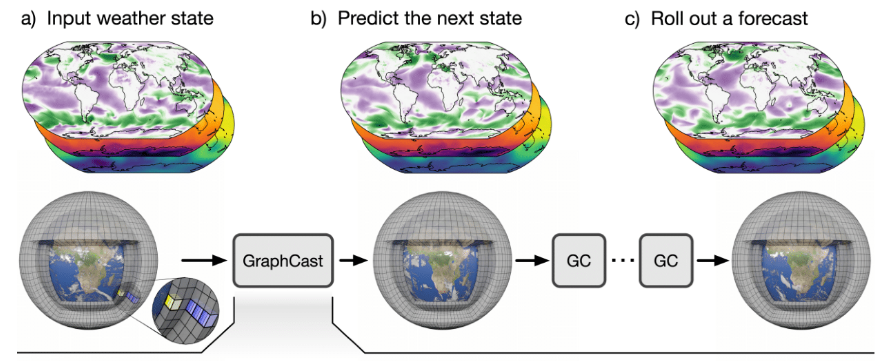
\includegraphics[width=0.9\textwidth]{images/GC1.png}
    \label{fig:image_graph}
\end{figure}
\begin{figure}[H]
    \centering
    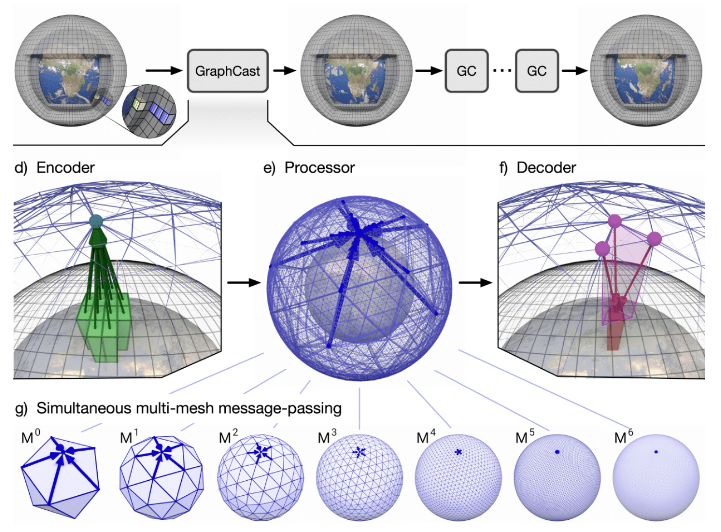
\includegraphics[width=0.9\textwidth]{images/GC2.png}
    \caption{Graph-Cast.}
    \label{fig:image_graph}
\end{figure}
